
The analysis relies on the selection of electrons, muons, jets and $b$-tagged jets. This chapter reviews the reconstruction, definition, efficiencies and calibration of these objects in ATLAS.

\section{Object reconstruction}\label{s:objects}
\subsection{Muons}
Muons are reconstructed by combining tracks found in the muon spectrometer and inner detector. Track segments are found in each layer of then detector then combined, taking into account energy loss while crossing the calorimeters. Tracks in the ID are required to pass minimum hit requirements in the Pixel, SCT, and TRT. Muons can be reconstructed using only the MS, but in this analysis uses \emph{combined} muons, reconstructed in both the MS and ID, to ensure high purity.

The muon reconstruction efficiency can be measured using the \emph{tag-and-probe} method. The ID reconstruction efficiency is determined from events reconstructed with one combined muon, the \emph{tag}, and a second muon only required to have an MS track, the \emph{probe}. The ID reconstructrion efficiency is given by the fraction of events where the MS track probe also has a track in the ID. The same method can be used to determine the efficiency of the MS reconstruction as matching. This time, the ID segements are used as the probe and the MS+matching efficiency is given by the fraction of ID segments with a matching MS segment. The overall muon reconstruction efficiency is given by the product of these two efficiencies. To obtain the scale factors (SF), the muon reconstruction efficiency in data and MC is compared: $SF = \epsilon_{data}/\epsilon{MC}$. These scale factors are applied to the simulation to ensure that muons are reconstructed with the same efficiency in MC as in data. For muons, the SFs are calculated in bins of \pt\ and $\eta$ for $Z\rightarrow \mu\mu$ and $J/\Psi\rightarrow \mu\mu$ events~\cite{muonpaper}. 

The muon momentum scale and resolution of the MC must also be corrected to match data. Differences can come from mismodeling of the detector geometry, magnetic field, or energy loss in the calorimeter. Scale factors are determined by comparing the shape of the energy distribution in $Z\rightarrow \mu\mu$ and $J/\Psi\rightarrow \mu\mu$ events. For 2012, the corrections were less than 0.1\%~\cite{muonpaper}.

Finally, the efficiency of the muon trigger is also estimated via the tag-and-probe method. In this analysis, the logical OR of two triggers is used to identify muons: a 24 GeV trigger with a loose track-based isolation requirement (the sum of the \pt of tracks within a cone of $\Delta R$=0.2 must be less than 12\% the \pt of the muon) and a 36 GeV trigger without an isolation requiment. For $\pt<100 \gev$, $Z\rightarrow\mu\mu$ events are used to estimate the trigger efficiency, while $W+$jets is used for \pt\ above this threshold. The muon trigger efficiency in the barrel region is derived from $Z\rightarrow\mu\mu$ events is shown in Figure~\ref{muontrigger}

\begin{figure}[h]
\centering
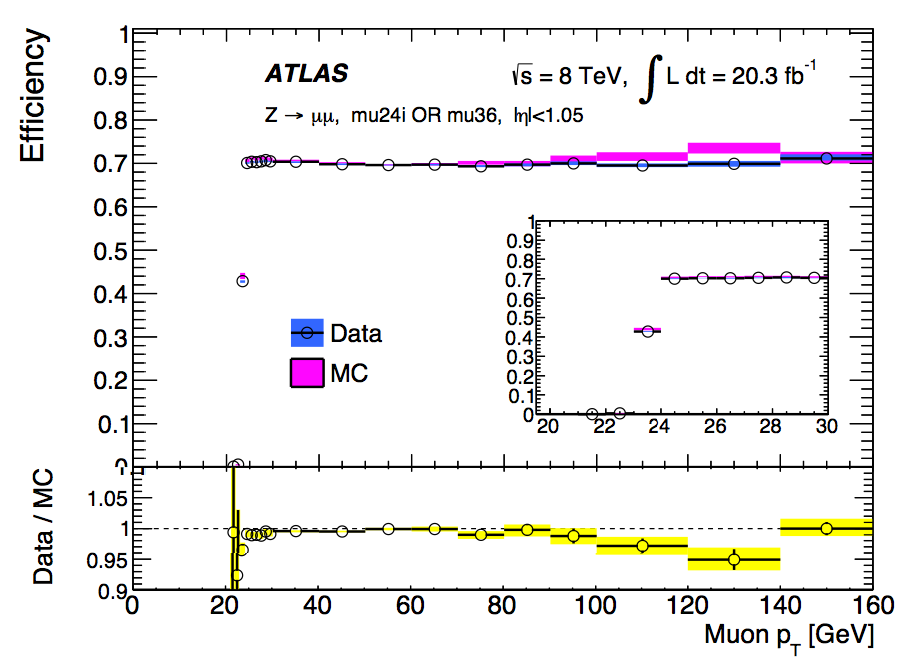
\includegraphics[width=0.6\textwidth]{fig/obj/muontrigger.png}
\caption{Reconstruction and identification efficiency~\cite{Aad:2014fxa}.}
\label{fig:muontrigger}
\end{figure}
\subsection{Electrons}




